\documentclass[xcolor=dvipsnames]{beamer}
\usepackage{graphicx,epstopdf}
\usepackage{fancyhdr}
\usepackage{cite}
\usepackage{graphicx, epstopdf}
\usepackage{amsmath}
\usepackage{array}
\usepackage{epsfig}
\usepackage{amssymb}
\usepackage{subfigure}
\usepackage[ruled, lined,linesnumbered]{algorithm2e}
\usepackage{algorithmic}
\usepackage{tabularx}
\usepackage{rotating, boxedminipage}
\usepackage{rotating,multirow}
\usepackage{float}
\usepackage{wrapfig}
\usepackage{algorithm2e}
\usetheme{Boadilla}
\usecolortheme[named=Blue]{structure}
\setbeamertemplate{items}[square]
\setbeamertemplate{caption}[numbered]
\setbeamertemplate{caption}[small]
\usepackage[absolute,overlay]{textpos}
\newenvironment{reference}[2]{%
  \begin{textblock*}{\textwidth}(#1,#2)
     \bgroup\fontsize{6pt}{\baselineskip}\selectfont\color[RGB]{0,112,192}}{\egroup\end{textblock*}}

\begin{document}
    \title[SSCI]{A Hybrid Estimation of Distribution Algorithm with Differential Evolution for Global Optimization}
    \author{Bing Dong}
    \institute[East China Normal University]{East China Normal University, Shanghai, China}
    \logo{
\includegraphics[height=0.5cm,width=3.0cm]{university-logo-ecnu}\vspace{230pt}}
    \date{\today}
    \begin{frame}
        \titlepage
    \end{frame}
    \setbeamertemplate{section in toc}[square]
    \begin{frame}
        \frametitle{Outline}
        \tableofcontents
    \end{frame}

    \section{Background}
    \begin{frame}
    \frametitle{Definition}
    The box-constrained continuous global optimization can be stated in the following:
    \begin{equation}
    \begin{array}{rl}
    \mbox{min} & f(x)\\
    \mbox{s.t} & x\in[a_i,b_i]^n
    \end{array}
    \label{MOP}
    \end{equation}

    \begin{itemize}
    \item $x=(x_1, x_2, \cdots, x_n)^T\in{R^n}$ is a decision vector
    \item $[a_i, b_i]^n$ is the search space
    \item $f:R^n\to{R}$ is the objective function
    \end{itemize}
    \end{frame}


    \begin{frame}
    \frametitle{DE}

    \begin{columns}
        \begin{column}{0.5\textwidth}
        \begin{figure}[H]
            \graphicspath{{figs/}}
            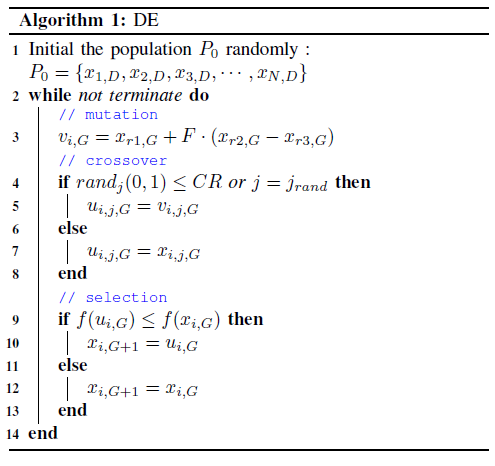
\includegraphics[width=0.9\textwidth]{de.png}
            \caption{The algorithm framework of DE}
        \end{figure}
    \end{column}
    \begin{column}{0.5\textwidth}
    \begin{itemize}\small
    \setlength\itemsep{0em}
      \item $N$ is the population size, and $D$ is the dimension of the target vector.
      \item At each generation $G$, a mutant vector $v_{i,G}$ is obtained by mutation. $F$ is the scaling factor, $r1, r2, r3$ are mutually different integers randomly selected from $[1,N]$.
      \item The trial vector $u_{i,j,G}$ is generated by combing $v_{i,G}$ and $x_{i,j,G}$. $rand_j(0,1)\in[0, 1]$ is a uniformly distributed random number, and $j_{rand}$ is a random integer between $j$ and $D$. $CR$ is the controlling parameter.
      \item $u_{i,G}$ and $x_{i,G}$ compete to enter the next generation in accordance with the objective function value.
    \end{itemize}
    \end{column}
    \end{columns}
    
    \end{frame}

    \begin{frame}
    \frametitle{EDA}
    \begin{columns}
        \begin{column}{0.5\textwidth}
        \begin{figure}[H]
            \graphicspath{{figs/}}
            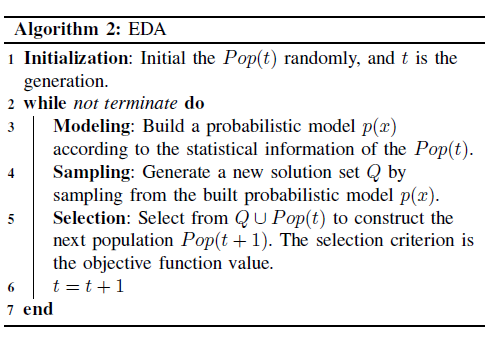
\includegraphics[width=0.9\textwidth]{eda.png}
            \caption{The algorithm framework of DE}
        \end{figure}
    \end{column}
    \begin{column}{0.5\textwidth}
    \begin{itemize}\small
    \setlength\itemsep{0em}
    \item $t$ is the generation counter.
    \item $Pop(t)=\{x^1,x^2, \cdots x^N\}$ is the population at generation $t$.
    \item $Q$ is a new solution set sampled from the probabilistic model.
    \end{itemize}
    \end{column}
    \end{columns}   
    \end{frame}


    \section{DE/EDA-EIG}
    \begin{frame}
    \frametitle{mutation scheme}
    \begin{figure}
    \centering
    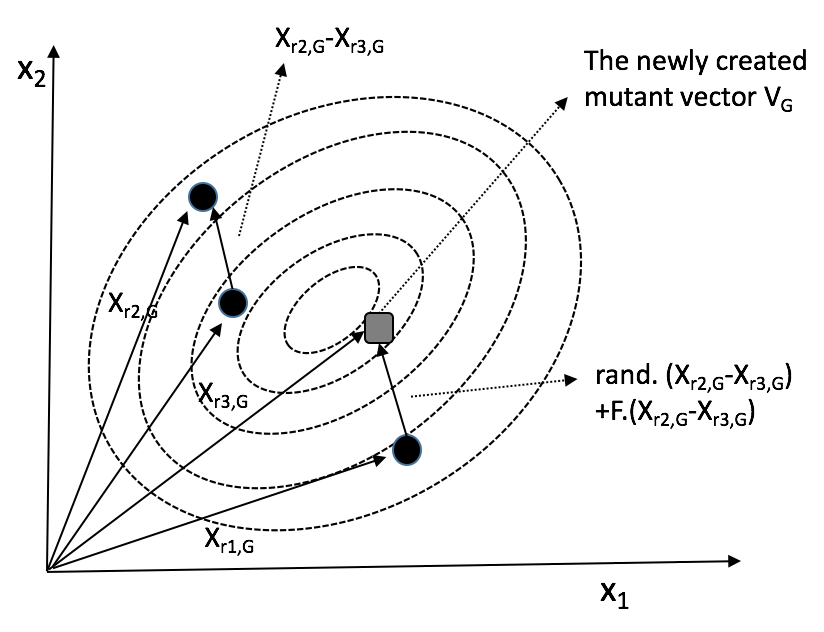
\includegraphics[width=0.3\columnwidth]{mutation1.png}
    \caption{The schema of the mutation}
    \end{figure}
    \begin{equation}
    \label{DE}
    X=X_{r_1}+rand\cdot(X_{r_2}-X_{r_3})+F\cdot(X_{r_2}-X_{r_3})
    \end{equation}

    \begin{itemize}
    \item $X_{r_1}$, $X_{r_2}$, $X_{r_3}$ are sampled randomly from the population
    \item $r_1$, $r_2$ and $r_3$ are mutually exclusive integers selected randomly from 1 to $NP$
    \item $F$ is the scaling factor
    \end{itemize}
    \end{frame}
    \begin{figure}
    \centering
    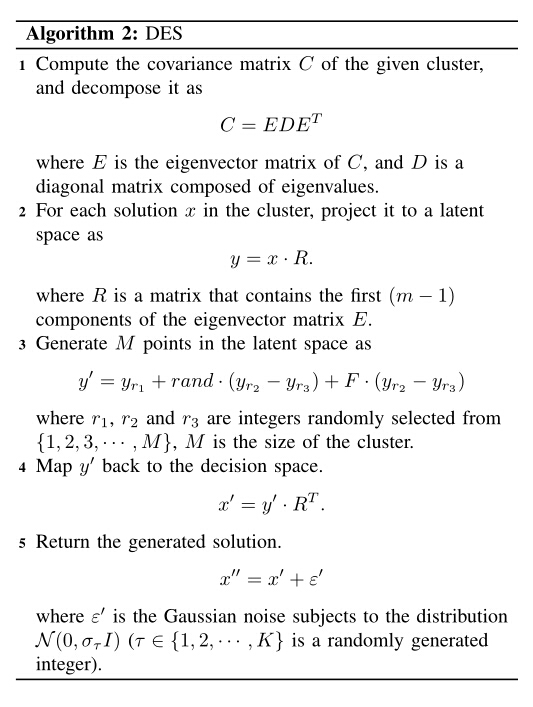
\includegraphics[width=0.5\columnwidth]{alg2.jpg}
    \caption{The framework of DES}
    \end{figure}

    \begin{frame}
    \begin{figure}
    \centering
    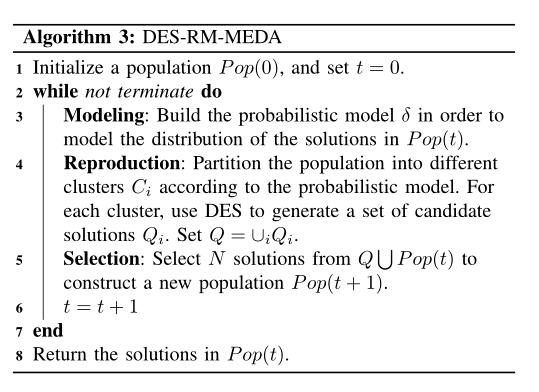
\includegraphics[width=0.5\columnwidth]{alg3.jpg}
    \caption{The framework of DES-RM-MEDA}
    \end{figure}
    \end{frame}
    \section{Experiment results}
    \begin{frame}
    \frametitle{Experimental settings}
    The 10 test instances, $F1-F10$, introduced in RM-MEDA are used as the benchmark problems.
    \begin{itemize}
    \item \emph{Initialization of the population}: The initial population in algorithms is randomly generated.
    \item \emph{The number of new trial solutions generated}: 100 for instances ($F3$, $F7$, $F9$), and 200 for other instances.
    \item \emph{The number of decision variables}: 30
    \item \emph{The number of clusters}: 5
    \item\emph{The scaling factor $F$}: 0.4
    \item\emph{The number of runs}: 30
    \item\emph{The number of generation}: 100 for instances ($F1$, $F2$, $F5$, $F6$), 200 for instances $F4$ and $F8$, and 1000 for instances $F3$, $F7$ and $F9$.
    \end{itemize}
    \end{frame}

    \begin{frame}
    \frametitle{The sensitivity of the F}
    \begin{figure}[htbp]
    \centering
    \subfigure[F1-F5]{\includegraphics[ width=4cm, height=3.2cm]{figs/f1_f5.eps}}
    \subfigure[F6-F9]{\includegraphics[ width=4cm, height=3.2cm]{figs/f6_f9.eps}}
    \subfigure[F10]{\includegraphics[ width=4cm, height=3.2cm]{figs/f10.eps}}
    \end{figure}
    \end{frame}

    \begin{frame}
    \frametitle{Wilcoxon's rank sum test}
    \begin{figure}
    \centering
    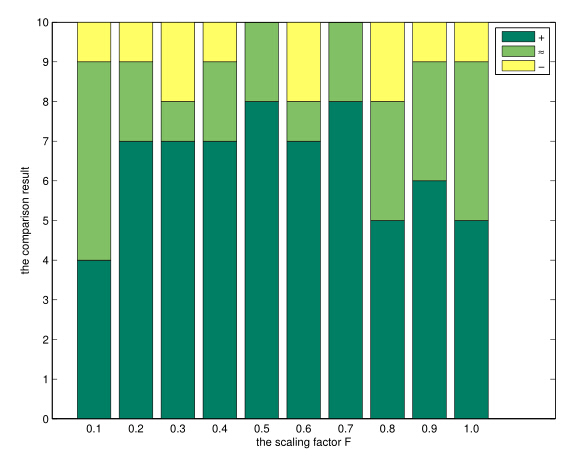
\includegraphics[width=0.6\columnwidth]{f_performance.jpg}
    \caption{The compariosn of RM-MEAD and RM-MEDA-DES with different settings of F}
    \end{figure}
    \end{frame}

    \begin{frame}
    \frametitle{Comparison study}
    \begin{figure}[htbp]
    \centering
    \subfigure[F1]{\includegraphics[ width=3.7cm, height=2.8cm]{figs/f1_igd.eps}}
    \subfigure[F2]{\includegraphics[ width=3.7cm, height=2.8cm]{figs/f2_igd.eps}}
    \subfigure[F3]{\includegraphics[ width=3.7cm, height=2.8cm]{figs/f3_igd.eps}}
    \subfigure[F4]{\includegraphics[ width=3.7cm, height=2.8cm]{figs/f4_igd.eps}}
    \subfigure[F5]{\includegraphics[ width=3.7cm, height=2.8cm]{figs/f5_igd.eps}}
    \caption{The dashed line is RM-MEDA, and the solid line is RM-MEDA-DES}
    \end{figure}
    \end{frame}

    \begin{frame}
    \frametitle{Comparison study}
    \begin{figure}[htbp]
    \centering
    \subfigure[F6]{\includegraphics[ width=3.7cm, height=2.8cm]{figs/f6_igd.eps}}
    \subfigure[F7]{\includegraphics[ width=3.7cm, height=2.8cm]{figs/f7_igd.eps}}
    \subfigure[F8]{\includegraphics[ width=3.7cm, height=2.8cm]{figs/f8_igd.eps}}
    \subfigure[F9]{\includegraphics[ width=3.7cm, height=2.8cm]{figs/f9_igd.eps}}
    \subfigure[F10]{\includegraphics[ width=3.7cm, height=2.8cm]{figs/f10_igd.eps}}
    \caption[small]{The dashed line is RM-MEDA, and the solid line is RM-MEDA-DES}
    \end{figure}
    \end{frame}

    \begin{frame}
    \frametitle{Comparison study}
    \begin{figure}
    \centering
    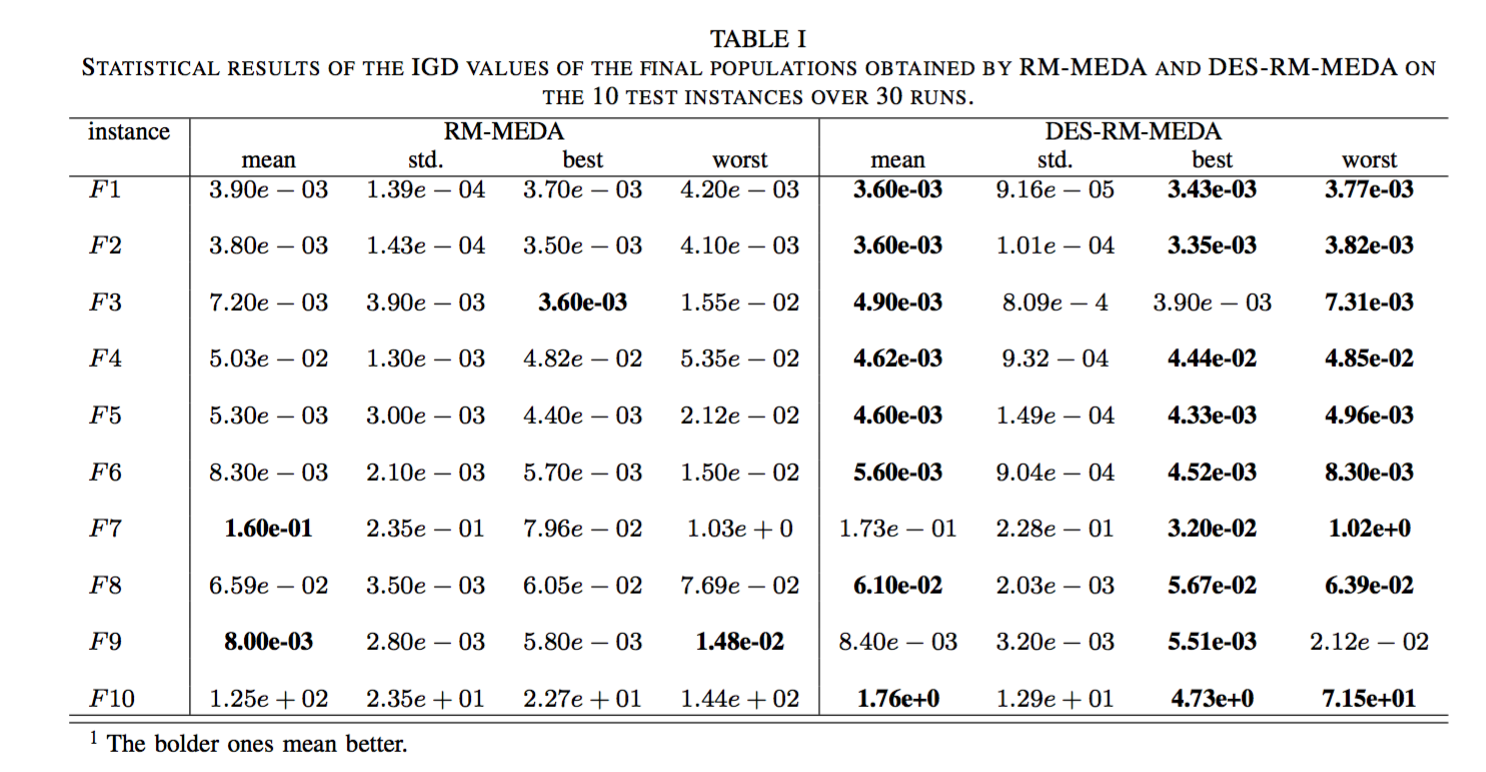
\includegraphics[width=1\columnwidth]{tab1.png}
    \end{figure}
    \end{frame}
    \section{Conclusions}
        \begin{frame}
        \frametitle{Conclusions}
        \textbf{Main contributions}
        \begin{itemize}
        \item A new sampling strategy for multiobjective estimation of distribution algorithm.
        \item Addressing to the issue of the extension scale setting in RM-MEDA.
        \end{itemize}
        This paper proposed a DES scheme to generate points in the latent space. The basic idea is to project the parent solutions
        into the latent space, and use a DE mutation operator to generate new points in the latent space based on the projected points, and finally map the points back to
        to the decision space added with Gaussian noise to generate offspring solutions. The DES is implemented into RM-MEDA to improve the performance. The results are impressive.
        \end{frame}

        \begin{frame}
        \frametitle{The future work}
       	\begin{itemize}
       	\item To exploit the deeper application of the DES. There is the possibility to apply the DES to other MOEAs.
       	\item It is valuable to explore the hybrid menthod of the DE and EDA. Though DE/EDA has been proposed, it is still interesting to explore the potential of this method.
       	And the arrange of the resources of DE and EDA is also an interesting topic.
       	\end{itemize}
       \end{frame}
    \section*{thx}
        \begin{frame}
        \begin{center}
        %\structure
        \fontsize{60pt}{\baselineskip}\selectfont \structure{Thanks!}
        \end{center}
        \begin{reference}{0mm}{80mm}
        \begin{itemize}
        \item  B. Dong, A. Zhou, and G. Zhang, A Hybrid Estimation of Distribution Algorithm with Differential Evolution for Global Optimization, 2016 IEEE Symposium Series on Computational Intelligence (SSCI), 2016.
        \end{itemize}
        \end{reference}
        \end{frame}
\end{document}
